%%%%%%%%%%%%%%%%%%%%%%%%%%%%%%%%%%%%%%%%%
% Beamer Presentation
% LaTeX Template
% Version 1.0 (10/11/12)
%
% This template has been downloaded from:
% http://www.LaTeXTemplates.com
%
% License:
% CC BY-NC-SA 3.0 (http://creativecommons.org/licenses/by-nc-sa/3.0/)
%
%%%%%%%%%%%%%%%%%%%%%%%%%%%%%%%%%%%%%%%%%

%----------------------------------------------------------------------------------------
%	PACKAGES AND THEMES
%----------------------------------------------------------------------------------------

\documentclass{beamer}

\mode<presentation> {

% The Beamer class comes with a number of default slide themes
% which change the colors and layouts of slides. Below this is a list
% of all the themes, uncomment each in turn to see what they look like.

%\usetheme{default}
%\usetheme{AnnArbor}
%\usetheme{Antibes}
%\usetheme{Bergen}
%\usetheme{Berkeley}
%\usetheme{Berlin}
%\usetheme{Boadilla}
%\usetheme{CambridgeUS}
%\usetheme{Copenhagen}
%\usetheme{Darmstadt}
%\usetheme{Dresden}
%\usetheme{Frankfurt}
%\usetheme{Goettingen}
%\usetheme{Hannover}
%\usetheme{Ilmenau}
%\usetheme{JuanLesPins}
%\usetheme{Luebeck}
\usetheme{Madrid}
%\usetheme{Malmoe}
%\usetheme{Marburg}
%\usetheme{Montpellier}
%\usetheme{PaloAlto}
%\usetheme{Pittsburgh}
%\usetheme{Rochester}
%\usetheme{Singapore}
%\usetheme{Szeged}
%\usetheme{Warsaw}

% As well as themes, the Beamer class has a number of color themes
% for any slide theme. Uncomment each of these in turn to see how it
% changes the colors of your current slide theme.

%\usecolortheme{albatross}
%\usecolortheme{beaver}
%\usecolortheme{beetle}
%\usecolortheme{crane}
%\usecolortheme{dolphin}
%\usecolortheme{dove}
%\usecolortheme{fly}
%\usecolortheme{lily}
%\usecolortheme{orchid}
%\usecolortheme{rose}
%\usecolortheme{seagull}
%\usecolortheme{seahorse}
%\usecolortheme{whale}
%\usecolortheme{wolverine}

%\setbeamertemplate{footline} % To remove the footer line in all slides uncomment this line
%\setbeamertemplate{footline}[page number] % To replace the footer line in all slides with a simple slide count uncomment this line

%\setbeamertemplate{navigation symbols}{} % To remove the navigation symbols from the bottom of all slides uncomment this line
}

\usepackage{graphicx} % Allows including images
\usepackage{booktabs} % Allows the use of \toprule, \midrule and \bottomrule in tables

%----------------------------------------------------------------------------------------
%	TITLE PAGE
%----------------------------------------------------------------------------------------

\title[GPR using MMF]{Summary of Recent Progress Applying MMF to Gaussian Process Regression} % The short title appears at the bottom of every slide, the full title is only on the title page

\author{Jon Eskreis-Winkler} % Your name
\institute[UChicago] % Your institution as it will appear on the bottom of every slide, may be shorthand to save space
{
University of Chicago \\ % Your institution for the title page
\medskip
\textit{eskreiswinkler@uchicago.edu} % Your email address
}
\date{\today} % Date, can be changed to a custom date

\begin{document}

\begin{frame}
\titlepage % Print the title page as the first slide
\end{frame}

\begin{frame}
\frametitle{Overview} % Table of contents slide, comment this block out to remove it
\tableofcontents % Throughout your presentation, if you choose to use \section{} and \subsection{} commands, these will automatically be printed on this slide as an overview of your presentation
\end{frame}

\section{What is a Gaussian Process?}% Sections can be created in order to organize your presentation into discrete blocks, all sections and subsections are automatically printed in the table of contents as an overview of the talk
%------------------------------------------------

% A subsection can be created just before a set of slides with a common theme to further break down your presentation into chunks

\begin{frame}
\frametitle{Gaussian Process motivation and definition}

\begin{itemize}
\item Given data $(\textbf{X}_n, \textbf{Y}_n)=(X_1, Y_1), \dots, (X_n, Y_n)$, how do you infer what type of process $f$ generated the data and responses? How do you enable predictions for future data?
\item The Bayesian approach uses  the posterior probability distribution for the process $f: \mathcal{X}^n \rightarrow \mathcal{Y}^n$ is 
$$P(f|\textbf{X}_n, \textbf{Y}_n) = \frac{P(\textbf{Y}_n|f, \textbf{X}_n)P(f)}{P(\textbf{Y}_n|\textbf{X}_n)}$$
\item What is the function space to which $f$ belongs? Need to restrict the space if we want to be able to measure the numerator terms.
\item Simplifying assumption: $f$ is a Gaussian Process.
\item A mapping $f$ is called a \textbf{Gaussian Process} if for any $m\in\mathbb{N}$, for any $m$-length  input set $(X_1, \dots, X_m)$, the distribution of $(f(X_1), \dots, f(X_m))$ is multivariate normal with $(f(X_1), f(X_2), \dots , f(X_n)) \sim N(\mu(x), K(x))$ with Mercer kernel $K$.
\end{itemize}
\end{frame}


\begin{frame}
\frametitle{Gaussian Process Intuition}
\begin{itemize}
\item Gaussian Process generalizes the notion of a finite dimensional Gaussian distribution to an infinite dimensional analog
$$X \sim \mathcal{N}(\mu, \Sigma) \Longleftrightarrow f(\textbf{X}_n) \sim \mathcal{N}(\mu(\textbf{X}_n), \Sigma(\textbf{X}_n))$$
The mean and covariance functions are defined by the data, assume $\mu(x)=0$ for simplicity.
\item For prediction, the covariance function $\Sigma_p(\textbf{X}_n)$ is often of the form $\Sigma(\textbf{X}_n) = K+\sigma^2I$.
\end{itemize}
\end{frame}

\begin{frame}
\begin{itemize}
\item The prior for $f$ is the density for an $n$-dimensional multivariate normal:
$$P(f(\textbf{X}_n)) = (2\pi)^{-\frac{n}{2}} \det( \Sigma(\textbf{X}_n))^{-\frac{1}{2}} \exp \left(-\frac{1}{2} f(\textbf{X}_n)^T\Sigma(\textbf{X}_n)^{-1} f(\textbf{X}_n) \right)$$
\item The likelihood of the data is the conditional distribution $\textbf{Y}_n |\textbf{X}_n \sim N(0, K(x) + \sigma^2 I)$ and log-likelihood is 
$$\log P(\textbf{Y}_n|\textbf{X}_n) = -\frac{n}{2} \log (2\pi) - \frac{1}{2} \log \det |K+\sigma^2I| -\frac{1}{2} \textbf{Y}_n^T (K+\sigma^2 I)^{-1} \textbf{Y}_n$$
\item To make predictions, we define the distribution for $Y_{n+1} | \textbf{X}_n, \textbf{Y}_n, X_{n+1}$
$$Y_{n+1} | \textbf{X}_n, \textbf{Y}_n, X_{n+1} \sim N(\tilde{\mu}(x), \tilde{\Sigma}(x))$$
where $\tilde{\mu} = k(X_{n+1},\textbf{X}_n)(K(x) + \sigma^2 I)^{-1} \textbf{Y}_n$ and $\tilde{\Sigma} = k(X_{n+1},X_{n+1}) - k(X_{n+1},\textbf{X}_n)(K(x) + \sigma^2 I)^{-1}k(\textbf{X}_n,X_{n+1})$.

\end{itemize}
\end{frame}

\subsection{Computational Bottleneck} 
\begin{frame}
\frametitle{Computational Bottleneck}
\begin{block}{Common computational complexities}
\begin{itemize}
\item Using Gauss-Jordan elimination, matrix inversion has complexity $O(n^3)$.
\item Finding determinant of a matrix by LU decomposition has complexity $O(n^3)$.
\end{itemize}
\end{block}
\begin{itemize}
\item For large $n$, this makes evaluation of the log-likelihood of the posterior and predictions using the posterior  intractable -- recall the inverse and determinant in the log-likelihood function and the inverse involved in prediction.
\item What can be done?
\end{itemize}

\end{frame}

\section{Potential for MMF to Help}
\begin{frame}
\frametitle{MMF Background}
\begin{itemize}
\item The MMF of a symmetric matrix $K$ is a multi-level factorization that approximates $A$
$$A \approx Q_1^T \cdots Q_L^T H Q_L \cdots Q_1$$
\item $H$ is a matrix which is approximately diagonal -- it is diagonal except for a "small" block of nonzero entries.
\item $Q_1, Q_2,\dots, Q_L$ are increasingly local rotations matrices, with a shrinking "active set" of rotations.
\end{itemize}
\end{frame}

\begin{frame}
\frametitle{Application of MMF to GPR Bottleneck}
Suppose that a MMF has been constructed for the matrix $(K+\sigma^2I)$
\begin{itemize}
\item  Determinant computation is only as complicated as computing the determinant of $H$. The computational cost is $O(nh^2)$ where $h$ is the dimension of $H$'s non-diagonal block. Also, $\forall i\in [1,L], \ \det(Q_i)=1$.
\item Matrix inversion is similarly simplified to $O(nh^2)$ because $\forall i \in [1,L], \ Q_iQ_i^T = I$ and $H^{-1}$ is reduced to inverting the non-diagonal block of $H$ and setting the remaining diagonal elements $d_{ii}$ of $H$ to be $\frac{1}{d_{ii}}$.
\item Similar to MMF, these procedures will thus scale roughly linearly with $n$, assuming $h$ is sufficiently small.
\end{itemize}
\end{frame}

\section{Application: Irish Wind Data}
\begin{frame}
\frametitle{Irish Wind Data}
\begin{itemize}
\item Daily average wind speeds for January 1961- December 1978 at 12 synoptic meteorological stations in the Republic of Ireland.
\item Excellent database for studying spacio-temporal aspects of a dataset. 
\item Good testbed for potential of MMF. There are (12 sites)(17 years)(365 days) = 74,460 total observations.
\end{itemize}
Haslett, J. and Raftery, A. E. (1989). Space-time Modelling with Long-memory Dependence: Assessing Ireland's Wind Power Resource (with Discussion). Applied Statistics 38, 1-50. 
\end{frame}
\begin{frame}
\frametitle{Irish Wind Data}
\begin{center}
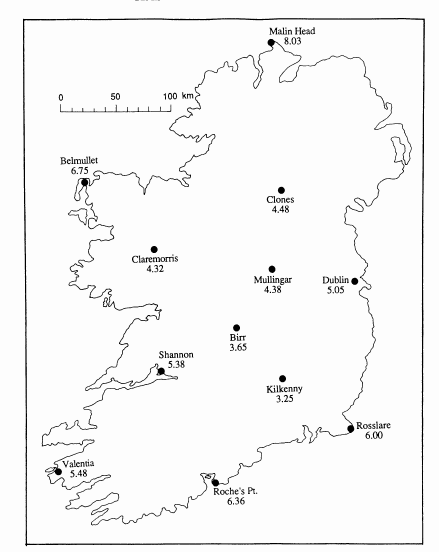
\includegraphics[scale=0.4]{fig1.png}
\end{center}
\end{frame}

\begin{frame}
\frametitle{Irish Wind Data}
\begin{center}
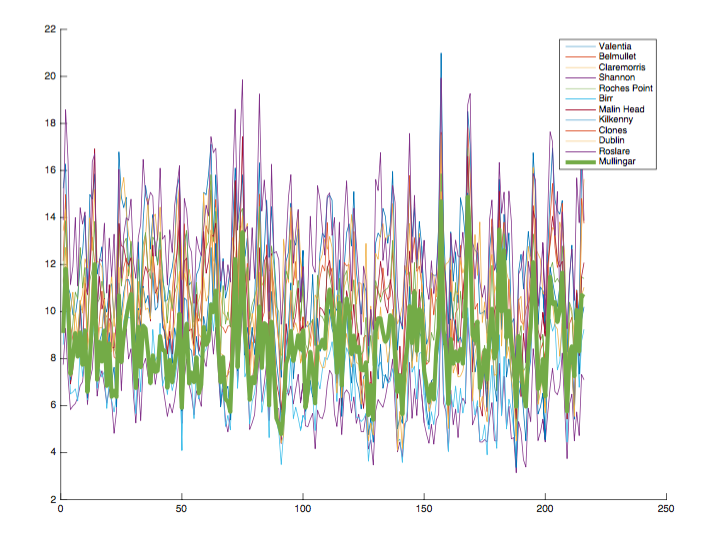
\includegraphics[scale=0.4]{fig3.png}
\end{center}
\end{frame}

\begin{frame}
\frametitle{Can we infer one station's measurements from the others'?}
\begin{itemize}
\item Training data are 17 years of measurements from all non-Mulligar stations
\item Test data is the Mullingar station's measurements.
\item To permit comparison with Matlab, needed to shrink data -- averaged over months.
\item 6 predictor variables: MonthID, Year, Month, Longitude, Lattitude, isCoastal (binary). Response is average monthly wind speed.
\item Use RBF kernel for Kernel matrix with varying length-scales:
$$K_{ij} = k(x_i, x_j)+\sigma_n^2\delta_{i,j} = \sigma_f^2 \exp(-\sum_{k=1}^6 \frac{(x_{i,k}-x_{j,k})^2}{l_i^2})+\sigma_n^2\delta_{i,j}$$
\end{itemize}
\end{frame}

\begin{frame}
\frametitle{Optimization}
\begin{itemize}
\item Need to find $\theta = (\sigma_f^2, \sigma_n^2, l)$ to maximize the log-likelihood of $p(\textbf{Y}_n|\textbf{X}_n)$.
\item Gradient descent is used to maximize log-likelihood, but used direct inverse because MMF determinant option was not yet available.
\item Performed a parameter search for $\theta_\mathrm{opt}$ by starting gradient descent on log-likelihood 20 times uniformly over a predefined "reasonable" parameter space. Procedure produced $\{\hat \theta^{(i)}\}_{i=1}^{20}$.
\item The predictions for all $\theta\in \{\hat \theta^{(i)}\}_{i=1}^{20}$ seemed very close so I simply averaged over their predictions.
\end{itemize}
\end{frame}

\begin{frame}
\frametitle{GPR Performance of MMF}
\begin{center}
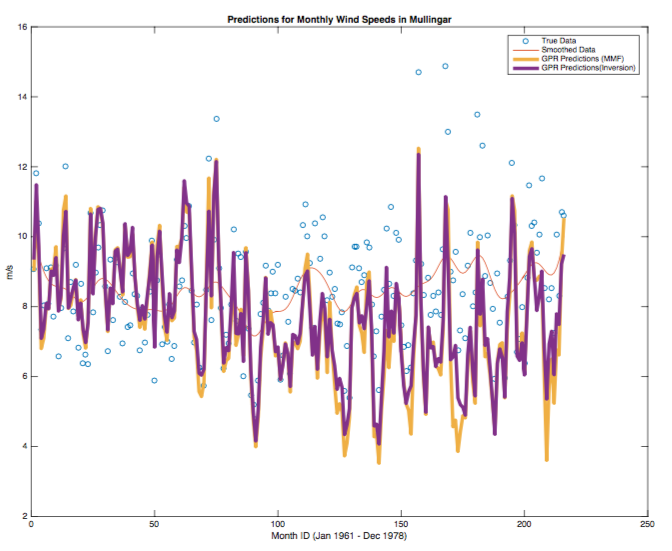
\includegraphics[scale=0.4]{fig2.png}
\end{center}
\end{frame}
\section{Conclusion}
\begin{frame}
\frametitle{Next Step}
\begin{itemize}
\item Improve parameter estimates by adding random restarts and by sampling more finely over the parameter space using a cluster.
\item Incorporate MMF into the parameter search -- not just prediction.
\item Develop connection between compression and prediction accuracy.
\end{itemize}
\end{frame}

\end{document} 